\section{A simple notcurses render\slash event loop}
I'm not typically a fan of example-based instruction, preferring to build things
up from formal axioms. Following chapters will effect such an approach. First,
however, let's work a semi-substantial example covering a varied set of
Notcurses routines. We're going to create seven planes, one for each kind
of tetrimino, and map an image file to the background. We'll add support for
switching between the pieces, rotating them, and sliding them around the
screen. Finally, we'll deal with collisions, and fluid handling of
screen resizings. In the course of doing so, you'll learn several important
Notcurses techniques:

\begin{denseitemize}
\item{Drawing and rotating these tetriminos will involve colors, gradients, and
      transparencies. The former are fundamental drawing tools. The latter is
      all one needs for sprites.}
\item{Mapping the background will involve image decoding, scaling, and blitting.}
\item{We'll cover most of what's worth knowing regarding input.}
\end{denseitemize}

This example will be picked up and further developed in the Tetris case study
of §~\ref{section:casestudy}\footnote{Were you aware that there is a standard
for Tetris clones? There is indeed\cite{tetris}.}.

\begin{figure}[!htbp]
\centering 
\includegraphics[width=.5\linewidth]{media/tetriminos.png}
\caption{Piping hot tetriminos, fresh from~\textit{Spiritus Mundi}.}
\label{fig:tetriminos}
\end{figure}

Almost every Notcurses program will take the same general form, an \textit{event+render loop}:

\begin{denseitemize}
\item{Essential screen elements are laid down.}
\item{Initial state is discovered and added to the display.}
\textbf{begin loop} 
\item{Some thread, perhaps the only thread in the process, watches
    for user input. Other threads might be collecting system events that will
    change the state. Either way, an event occurs.}
\item{Thread(s) receiving events perform any necessary mutual exclusion.}
\item{Thread(s) manipulate the Notcurses virtual state via \texttt{ncplane} manipulations.}
\item{\texttt{notcurses\_render()} is called by a single thread.}
\textbf{end loop}
\item{The process terminates.}
\end{denseitemize}

\subsection{Example: moving tetriminos with a keyboard}

We could load the pieces as images from files, but given the simplicity of the
sprites, it feels simpler to just hardcode them in our source. I don't want to
leave my text editor\footnote{Vim. See Figure~\ref{fig:xeroxemacs}.} to muck
with images when we can do everything in fewer than ten lines, even in a naïve
and wasteful encoding (Listing~\ref{list:tetrimino-data}).

\begin{listing}[!htbp]
\inputminted[]{C}{code/tetrimino-data.h}
\caption{The seven canonical tetriminos (from~\texttt{tetrimino.c}).}
\label{list:tetrimino-data}
\end{listing}

To warm up and get limber, let's create seven \texttt{ncplane}s, one for each type
of tetrimino. We'll lay them out in a 2-3-2 formation. This layout will be
sloppy, for now: our function
\texttt{tetrimio\_plane()} accepts a piece ID and a coordinate.
The plane it creates has its origin at this coordinate.
We're not yet adjusting for the size of the planes themselves when coming
up with these coordinates---this shifts everything down and to the right from
symmetric divisions of the screen, as you'll see.

\begin{figure}[!htbp]
\centering 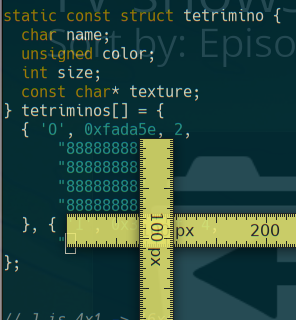
\includegraphics[width=.5\linewidth]{media/screenruler.png}
\caption{Font aspect ratios center around 0.5.}
\label{fig:aspectratio}
\end{figure}

We use two display rows per game row but four display columns per game column.
This reflects what is, at least on my display and font, pretty much a 0.5
aspect ratio (Figure~\ref{fig:aspectratio}).

\begin{listing}[!htbp]
\inputminted[]{C}{code/tetrimino-display.h}
\caption{Creating a single tetrimino (from~\texttt{tetrimino.c}).}
\label{list:tetrimino-display}
\end{listing}

There are a few essential things to
take away from Listing~\ref{list:tetrimino-display}:

\begin{denseitemize}
\item{Each time we call \texttt{ncplane\_putsimple()}, the cursor is advanced
      the expected amount. If we were calling \texttt{ncplane\_putegc()} with
      a multicolumn grapheme cluster, the cursor would be advanced multiple
      columns.}
\item{Between rows, we need move the cursor ourselves, since we're skipping over
      part of the plane (this isn't true for several of the pieces, but the
      cursor update is a trivial operation, not worth avoiding).}
\item{The cursor is always initialized to the origin of a new plane, and coordinates
      supplied to \texttt{ncplane\_} functions are relative to the plane,
      \textit{not} the terminal. Coordinates can be translated among planes
      using \texttt{ncplane\_translate()}.}
\item{We only have ASCII characters in the textures right now. Were we to
      introduce any multibyte UTF-8---and we may well do so, for e.\ g.\ the
      Box Drawing Characters---the \texttt{strlen()} we size our rows by here
      would no longer fly. We'd need use \texttt{mbstowcs()}, or redefine the
      textures as \texttt{wchar\_t} arrays and use \texttt{wcslen()},
      or change up our encoding\footnote{We go with the third option, as you'll see.}. \textfrench{\textit{Rien n'est simple, mais tout est facile\ldots}}}
\end{denseitemize}

\begin{listing}[!htbp]
\inputminted[]{C}{code/tetrimino-draw.h}
\caption{Distributing the tetriminos with ``flying-v'' technique (from~\texttt{tetrimino.c}).}
\label{list:tetrimino-draw}
\end{listing}

\begin{listing}[!htbp]
\inputminted[]{C}{code/tetrimino-main.h}
\caption{A one-shot, display-only \texttt{main()} (from~\texttt{tetrimino.c}).}
\label{list:tetrimino-main}
\end{listing}

Our \texttt{main()} sets the locale, initializes the terminal, and draws the
seven pieces (Listings~\ref{list:tetrimino-draw} and~\ref{list:tetrimino-main}).
Each piece has a one-letter name; for now, we draw with those glyphs. The
pieces are monochromatic. This renders familiar shapes in the correct colors
(Figure~\ref{fig:tetriminos-1}), but other than that, it's (like most classic
Curses programs) kinda fugly. I wouldn't want to play with these pieces.

\begin{figure}[!htbp]
  \centering
  \begin{minipage}{0.30\textwidth}
    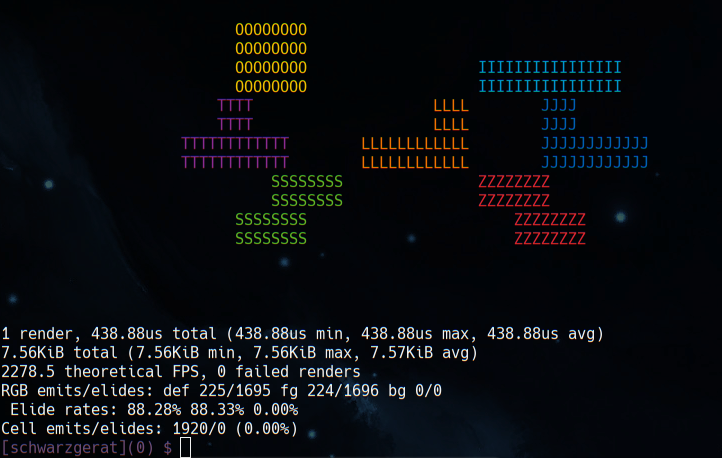
\includegraphics[width=1\linewidth]{media/tetriminos-1.png}
    \caption{Unspeakably foul.}
    \label{fig:tetriminos-1}
  \end{minipage}\hfill
  \begin{minipage}{0.30\textwidth}
    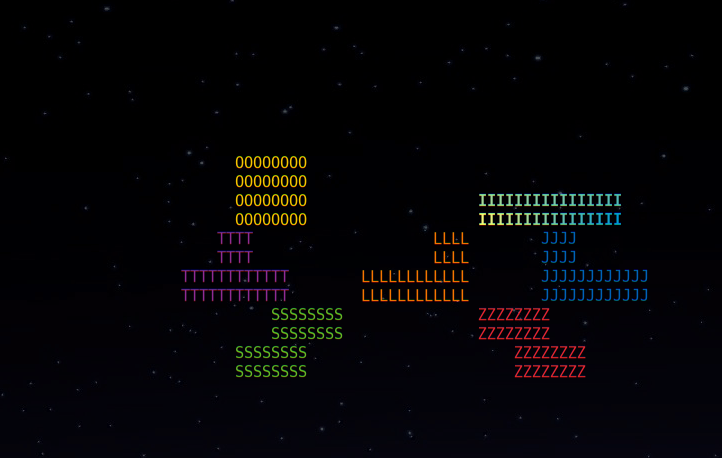
\includegraphics[width=1\linewidth]{media/tetrimino-gradient1.png}
    \caption{Adding a gradient.}
  \end{minipage}\hfill
  \begin{minipage}{0.30\textwidth}
    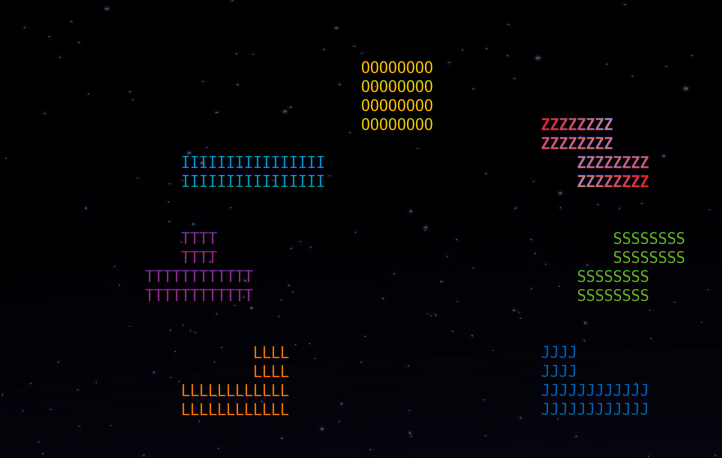
\includegraphics[width=1\linewidth]{media/tetrimino-gradient2.png}
    \caption{Linear expansion.}
  \end{minipage}\hfill
\end{figure}

This is hardly a render/event loop; in fact it's not a loop at all. If we were
using the alternate screen, we wouldn't see our output before flashing back to
the normal screen. Let's go ahead and hook up input. We'll be controlling one
of the tetriminos at a time---the selected piece will use boldface, and have its
color brightened\footnote{Note how we use two distinct indicators. On a monochromatic
display, we need the bold, and on a display which can't do bold, maybe we get a
color difference. Also, we want bold even if we have color, because until we
see the base color, there's no reason to think of the initial selection as
``bright''.}. We do so (Listing~\ref{list:tetrimino-switch}) with a pair of
helpers---\texttt{reduce()} and \texttt{highlight()}--- which drive the common
\texttt{blast()}. \texttt{blast()} makes use of two new functions,
\texttt{ncplane\_format()} and \texttt{ncplane\_stain()}. They allow the
attributes and channels, respectively, of a rectangular region to be changed
without altering other components. The corresponding glyph-only output routines
are likewise described in (Chapter~\ref{sec:staining}).

\begin{listing}[!htbp]
\inputminted[]{C}{code/tetrimino-switch.h}
\caption{Switching between pieces (from~\texttt{tetrimino-input.c}).}
\label{list:tetrimino-switch}
\end{listing}

While we're making things prettier, let's replace
those letters with some classy box-drawing characters, and improve on this
layout. We can do some simple algebraic extensions and get some linear spacing,
but it's just as easy to use trigonometric functions and get an approximation
to a circle. This is especially valuable as the terminal geometry changes; our
fixed linear scalings would break down as the display aspect changes, but a
good ol' circle will work on any sufficient radius
(Listing~\ref{list:tetrimino-drawcircle}).

\begin{listing}[!htbp]
\inputminted[]{C}{code/tetrimino-drawcircle.h}
\caption{Trigonometric layout: simpler, yet more accurate (from~\texttt{tetrimino-input.c}).}
\label{list:tetrimino-drawcircle}
\end{listing}

Since there's nothing else going on, it's trivial to process \texttt{stdin} in
a blocking fashion from our main thread. Let's add the code to track a selected
piece, visually highlight it, and process input (Listing~\ref{list:tetrimino-inputcore}).
The space bar will advance among the pieces in one direction,
and Tab in the other. The arrow keys and vi keys will translate the selected
piece in four directions. The parentheses will rotate the piece $\frac{\pi}{2}$ radians
clockwise and counterclockwise.

\begin{listing}[!htbp]
\inputminted[]{C}{code/tetrimino-inputcore.h}
\caption{Core input dispatch (from~\texttt{tetrimino-input.c}).}
\label{list:tetrimino-inputcore}
\end{listing}

Of course, when there's no other activity, things are easy. Quite often, we'll
have some periodic concurrent activity. Let's say we wanted to make the non-selected
tetriminos slowly rotate. The rotation isn't difficult; Notcurses provides
that functionality for you. But you don't want the rotation synced to input
activity, and you're hardly the kind of know-nothing what-not that would
busy loop on a nonblocking input interface, right? I hope you don't consider
yourself ``green'' if that's the case, because you're burning dinosaurs out
of sheer laziness. Let's do it right. There are of course four canonical
solutions to the problem of interleaving a set of asynchronous file descriptor-based
inputs against a set of periodic requirements; let's refresh ourselves:

\begin{denseitemize}
\item{No holds barred, take no prisoners state machine. No quarter asked and
    none given. Certainly the most \textit{enjoyable} choice of the four, the
    one closest to the nature of the machine, and the option with the most
    built-in job security. Casting off the crutch of the process scheduler, we
    execute in a single thread, carefully programming our
    \texttt{epoll()}\cite{epoll7} or \texttt{kqueue()}\cite{kqueue2} timeouts
    against a hierarchal, hashed timer wheel\cite{timerwheels}. As Alan Cox
    said, ``Computers are state machines. Threads are for people who don't
    understand state machines.''\footnote{Or did he? I can't find the original
    to cite. I wonder what the hell happened to Alan Cox.} Limited to a single
  CPU\ldots\ which probably isn't a problem here, but isn't exactly a great foundation
  on which to build our cathedral, \textfrench{\textit{n'est-ce pas?}}.}
\item{Two threads enter, one thread \texttt{exit()}s (hehehehe). We block on
    async I/O in our main thread. Another thread runs a timer wheel---for this,
    a loop around a \texttt{clock\_nanosleep()} will suffice. They
    lock against one another to avoid corrupting the screen or otherwise
    embarassing ourselves. The solution reeks of Java, but will work well
    enough, and any programmer---maybe even a Java programmer---ought be able
    to walk in and pick it up.}
\item{POSIX signaled timers. Noooooooooooooooooooooooooooooooooooooo.}
\item{Timer I/O multiplexing. Probably the best solution for a program of true
    scope, and in no way unfit for the task at hand. On Linux, you'll want
    \texttt{timerfd\_create()} and friends. On FreeBSD, look for \texttt{EVFILT\_TIMER}.
    Throw that into the appopriate I/O multiplexor call, spin it out among a
    few threads if you feel so inclined\cite{libtorque}, and call it a day.
  The only real disadvantage here is a lack of portability.}
\end{denseitemize}

Some will ask, ``Sounds dank, but what about on this shiny operating system I
purchased from Applooglesoft? Look, I can speak to it! Sirana, diminish my
freedoms and spy on me!'' I could give two shits about your closed-source
operating system. I presume you can purchase cloud-based Timers as a Service
(TaaS) or something.

We can now cycle through the pieces, and move the piece we've selected around
on the screen. Grab one and move it towards another piece. Experimentation will
reveal that each piece has a~\gls{boundingbox}, that there is a total ordering
among the seven pieces, and that a piece below another piece's bounding box is
robbed of its color (Figure~\ref{fig:tetrimino-badplane}). Recall from
Chapter~\ref{sec:rendering} how we solve for each coordinate of the display
grid: the EGC is a dimension distinct from the coloring channels. Each of the
planes we create is rectilinear, with the piece drawn using Unicode
\texttt{U+2588 FULL BLOCK}, and the other cells left unwritten. The foreground
for our pieces is an RGB color, and for the other cells is the default terminal
color. Upon intersecting with a lower plane, the lower plane's EGC is chosen for
rendering, but the foreground color is default terminal color (white in my
example). So the piece underneath flipping to white while another piece is
nearby makes perfect sense. The solution is simple: we set the foreground
transparent for the base character of each plane. Foreground calculation will
now bypass the plane where we haven't drawn, and the distorted plane regains
its expected colors (Figure~\ref{fig:tetrimino-trans}).

\begin{figure}[!htbp]
  \centering
  \begin{minipage}{0.30\textwidth}
    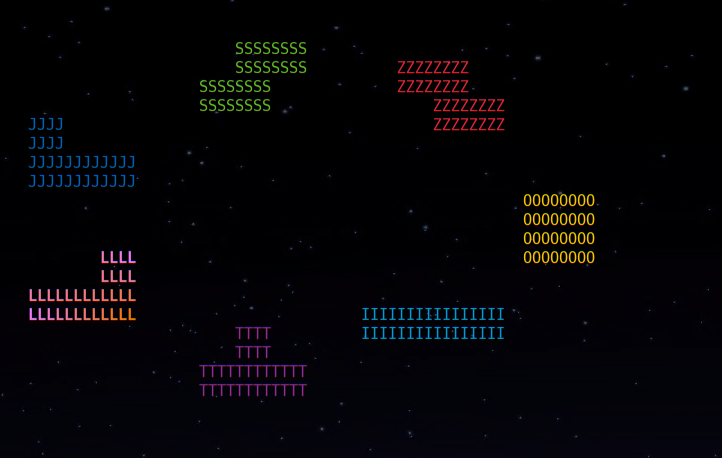
\includegraphics[width=1\linewidth]{media/tetrimino-gradient3.png}
    \caption{Trigonometry!}
  \end{minipage}\hfill
  \begin{minipage}{0.30\textwidth}
    
\includegraphics[width=1\linewidth]{media/tetrimino-gradient4.png}
    \caption{Unicode Blocks.}
  \end{minipage}\hfill
  \begin{minipage}{0.30\textwidth}
    
\includegraphics[width=1\linewidth]{media/tetrimino-gradient5.png}
    \caption{Better blocks.}
  \end{minipage}\hfill
\end{figure}

\begin{figure}[!htbp]
  \begin{minipage}{0.30\textwidth}
    
\includegraphics[width=1\linewidth]{media/tetrimino-gradient6.png}
    \caption{Adjusting for cell aspect ratio.}
  \end{minipage}\hfill
  \begin{minipage}{0.30\textwidth}
    
\includegraphics[width=1\linewidth]{media/tetrimino-gradient7.png}
    \caption{Undesirable plane interaction.}
    \label{fig:tetrimino-badplane}
  \end{minipage}\hfill
  \begin{minipage}{0.30\textwidth}
    
\includegraphics[width=1\linewidth]{media/tetrimino-gradient8.png}
    \caption{Resolve it with transparent planes.}
    \label{fig:tetrimino-trans}
  \end{minipage}\hfill
\end{figure}

\begin{listing}[!htbp]
\inputminted[]{C}{code/tetrimino-databox.h}
\begin{minted}{C}

\end{minted}
\inputminted[]{C}{code/tetrimino-displayutf8.h}
\caption{Improving appearance with Unicode Block Elements (from~\texttt{tetrimino-input.c}).}
\label{list:tetrimino-displayutf8}
\end{listing}

Adding a background image is simple. We'll render it to the standard plane, our
``background'' for now (remember, newly created planes are placed at the top of
the z axis). Despite decoding the image \textit{after} creation of the pieces,
the pieces are thus not hidden. There is no need to inform Notcurses of the
image's format, or parameters thereof; just provide the file name and target
rendering plane, and we're off. See Chapter~\ref{sec:libav} for a full treatment
of multimedia in Notcurses.

\begin{listing}[!htbp]
\inputminted[]{C}{code/tetrimino-background.h}
\caption{Throwing in a background (from~\texttt{tetrimino-input.c}).}
\label{list:tetrimino-background}
\end{listing}

To rotate the unselected pieces, we'll go ahead and spawn a POSIX thread. We'll
thus need lock against piece selection. We've been leaving all the end-of-process
cleanup in the capable hands of~\texttt{notcurses\_stop()}, but it can't go
terminating threads for us, and it in any case wouldn't be safe to do so while
said thread was calling into Notcurses! We'll use POSIX
cancellation\footnote{Which isn't anywhere near as bad as it's sometimes made out to be.
Find the places where you don't want to be cancelled. Each such place needs a
cleanup handler pushed/popped around it, or cancellation disabled for its
breadth. Things get a little counterintuitive with
cancellable-but-uninterruptible system calls, but that's nothing if you came up
on BSD signals. It's hardly the most offensive wart on the great hairy ass
that is ANSI/ISO C, and---heresy, I know---I honestly prefer (most of) the
POSIX model to (most of)
the threading introduced in \CC11.} to blast the rotator thread, and~\texttt{pthread\_join()}
it to ensure safe passage through shutdown.

\begin{listing}[!htbp]
\inputminted[]{C}{code/tetrimino-thread.h}
\caption{Spin them doggies (from~\texttt{tetrimino-input.c}).}
\label{list:tetrimino-thread}
\end{listing}

As a final touch, let's slide a dark, translucent plane underneath the
selected piece, making it more visible. We create this plane prior to the
pieces, ensuring it's below all of them (but above the background). We set it
black, and its alpha to \texttt{CELL\_ALPHA\_BLEND}. This way it won't entirely
block out the background underneath the selected piece, but it will dim it,
its black blending into the grey tones underneath. The piece is unaffected.

\begin{listing}[!htbp]
\inputminted[]{C}{code/tetrimino-box.h}
\caption{Set the selection off with a coaster (from~\texttt{tetrimino-input.c}).}
\label{list:tetrimino-box}
\end{listing}

\begin{figure}[!htbp]
  \centering
  \begin{minipage}{0.30\textwidth}
    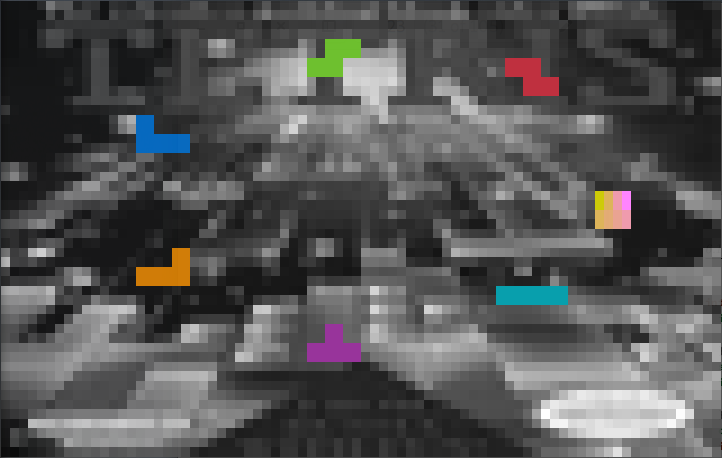
\includegraphics[width=1\linewidth]{media/tetrimino-bg.png}
    \caption{Background image, greyscaled.}
    \label{fig:tetrimino-bg}
  \end{minipage}\hfill
  \begin{minipage}{0.30\textwidth}
    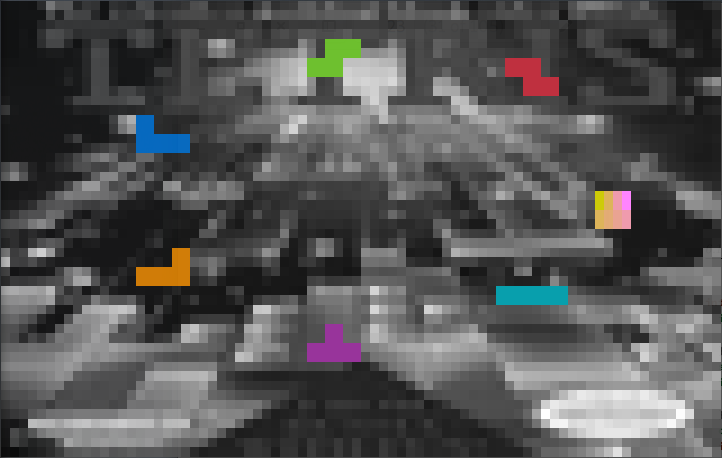
\includegraphics[width=1\linewidth]{media/tetrimino-bg.png}
    \caption{Opaque highlight box\textbf{FIXME}.}
  \end{minipage}\hfill
  \begin{minipage}{0.30\textwidth}
    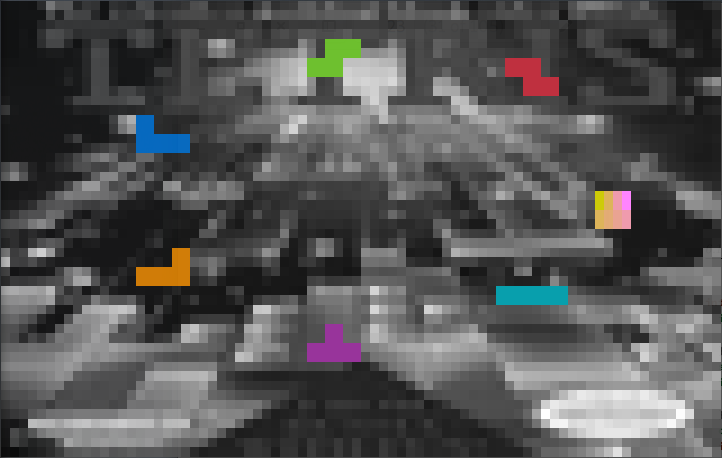
\includegraphics[width=1\linewidth]{media/tetrimino-bg.png}
    \caption{Rotation thread enabled\textbf{FIXME}.}
  \end{minipage}\hfill
\end{figure}

\begin{listing}[!htbp]
\inputminted[]{C}{code/tetrimino-inputmain.h}
\caption{Putting it all together (from~\texttt{tetrimino-input.c}).}
\label{list:tetrimino-inputmain}
\end{listing}
